\documentclass[a4paper,14pt]{extreport} % формат документа

\usepackage{amsmath}
\usepackage{cmap} % поиск в ПДФ
\usepackage[T2A]{fontenc} % кодировка
\usepackage[utf8]{inputenc} % кодировка исходного текста
\usepackage[english,russian]{babel} % локализация и переносы
\usepackage[left = 2cm, right = 1cm, top = 2cm, bottom = 2 cm]{geometry} % поля
\usepackage{listings}
\usepackage{graphicx} % для вставки рисунков
\usepackage{amsmath}
\usepackage{float}
\usepackage{multirow}
\graphicspath{{pictures/}}
\DeclareGraphicsExtensions{.pdf,.png,.jpg}
\newcommand{\anonsection}[1]{\section*{#1}\addcontentsline{toc}{section}{#1}}

\lstset{ %
	language=Lisp,                % Язык программирования 
	numbers=left,                   % С какой стороны нумеровать          
	frame=single,                    % Добавить рамку
}

\begin{document}
\begin{titlepage}

    \begin{table}[H]
        \centering
        \footnotesize
        \begin{tabular}{cc}
            \multirow{8}{*}{
\includegraphics[scale=0.35]{bmstu.jpg}}
            & \\
            & \\
            & \textbf{Министерство науки и высшего образования Российской Федерации} \\
            & \textbf{Федеральное государственное бюджетное образовательное учреждение} \\
            & \textbf{высшего образования} \\
            & \textbf{<<Московский государственный технический} \\
            & \textbf{университет имени Н.Э. Баумана>>} \\
            & \textbf{(МГТУ им. Н.Э. Баумана)} \\
        \end{tabular}
    \end{table}

    \vspace{-2.5cm}

    \begin{flushleft}
        \rule[-1cm]{\textwidth}{3pt}
        \rule{\textwidth}{1pt}
    \end{flushleft}

    \begin{flushleft}
        \small
        ФАКУЛЬТЕТ
        \underline{<<Информатика и системы управления>>\ \ \ \ \ \ \ 
        \ \ \ \ \ \ \ \ \ \ \ \ \ \ \ \ \ \ \ \ \ \ \ \ \ \ \ \ \ \ \ 
    \ \ \ \ \ \ \ \ \ \ \ \ \ \ \ } \\
        КАФЕДРА
        \underline{<<Программное обеспечение ЭВМ и
        информационные технологии>>
        \ \ \ \ \ \ \ \ \ \ \ \ \ \ \ \ \ \ \ \ }
    \end{flushleft}

    \vspace{2cm}

    \begin{center}
        \textbf{Лабораторная работа № 2} \\
        \vspace{0.5cm}
    \end{center}

    \vspace{4cm}

    \begin{flushleft}
        \begin{tabular}{ll}
            \textbf{Дисциплина} & Моделирование.  \\
            \textbf{Тема} & Функции распределения и функции плотности распределения.  \\
            \\
            \textbf{Студент} & Сиденко А.Г. \\
            \textbf{Группа} & ИУ7-73Б \\
            \textbf{Оценка (баллы)} & \\
            \textbf{Преподаватель} & Рудаков И.В.   \\
        \end{tabular}
    \end{flushleft}

    \vspace{4cm}

   \begin{center}
        Москва, 2020 г.
    \end{center}

\end{titlepage}

\begin{enumerate}

\item \textbf{Условие. }

Написать программу, для построения графиков функции и плотности для следующих распределений:
\begin{itemize}
\item равномерное распределение;
\item нормальное распределение. 
\end{itemize}

\item \textbf{Теория. }

\textbf{Равномерное распределение. }

Плотность распределения:

\begin{equation*}
f_X(x) = \left\{
\begin{matrix}
{1 \over b-a}, & x\in [a,b] \\
0, & x\not\in [a,b]
\end{matrix}
\right..
\end{equation*}

Функция распределения:

\begin{equation*}
F_X(x) \equiv P(X \le x) = \left\{
\begin{matrix}
0, & x < a \\
\dfrac{x-a}{b-a}, & a \le x < b \\
1, & x \ge b
\end{matrix}
\right..
\end{equation*}

 \textbf{Нормальное распределение. }
 
 Плотность распределения:

\begin{equation*}
 f(x) = \frac{1}{\sigma\sqrt{2\pi}}\; e^{ -\frac{(x-\mu)^2}{2\sigma^2} }
 \end{equation*}
 
 Функция распределения:

\begin{equation*}
 F(x) = \frac 1 {\sigma\sqrt{2\pi}} \int\limits_{-\infty}^{x} e^{ -\frac{(t-\mu)^2}{2\sigma^2}} \, dt
 \end{equation*}
 
\item \textbf{Полученные результаты. }

 Ниже на графиках представлены результаты работы программы, так же указаны значения $\mu, \sigma, a, b$, которые использовались для построения. 

\begin{figure}[H]
  \centering
  \caption{Пример 1. }
  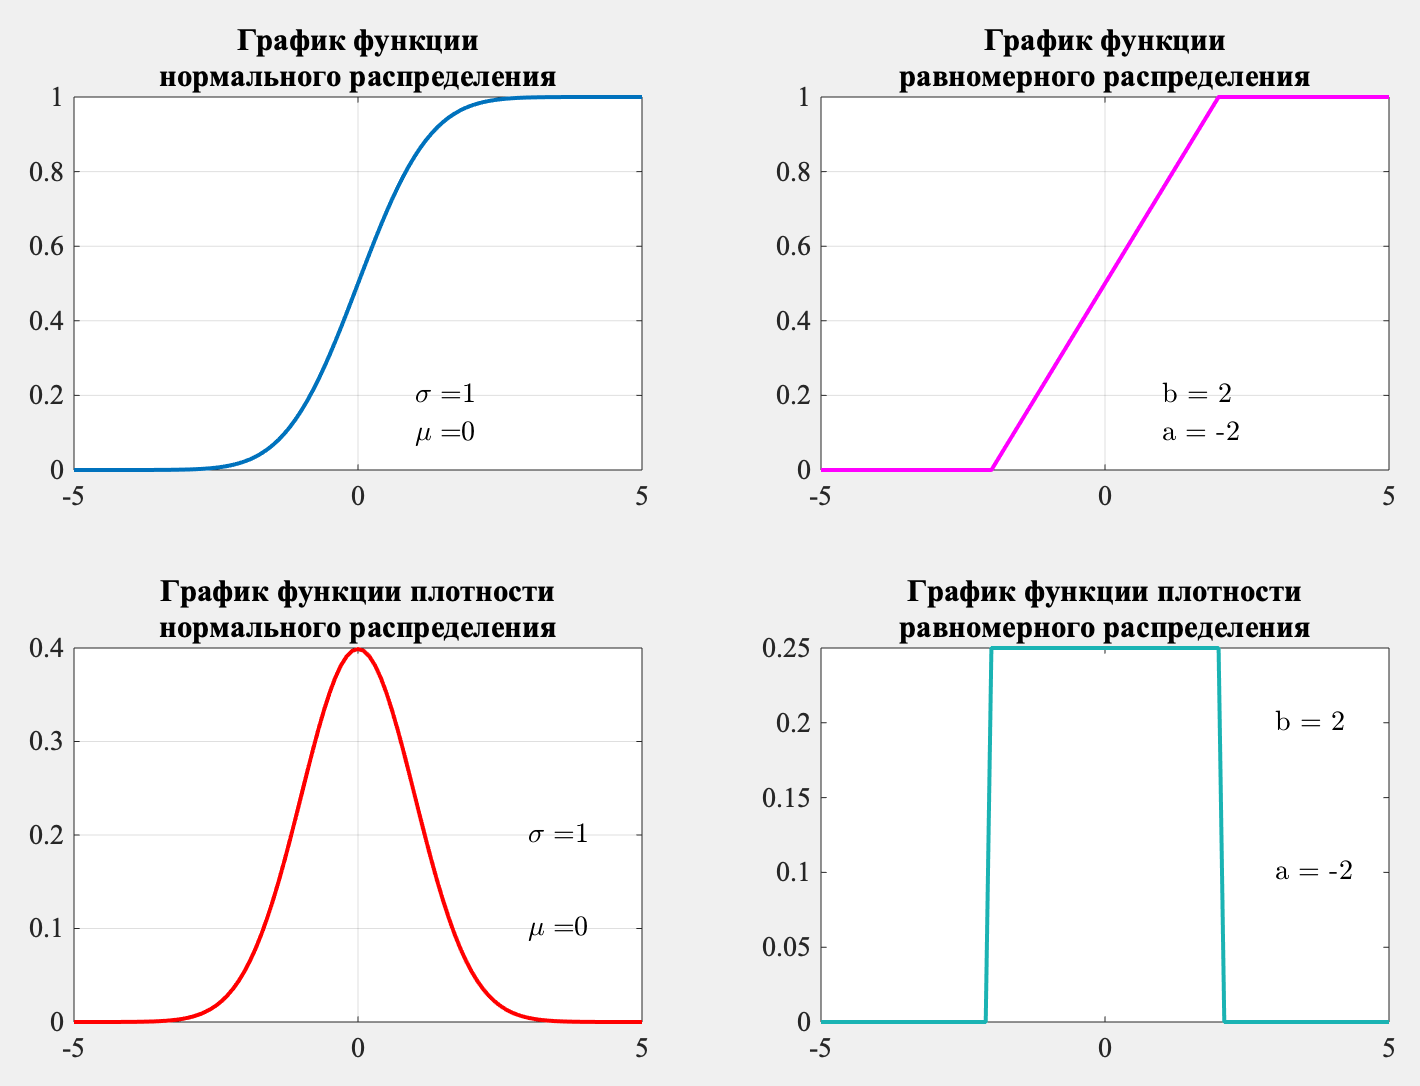
\includegraphics[scale=0.6]{2}
\end{figure}

\begin{figure}[H]
  \centering
  \caption{Пример 2. }
  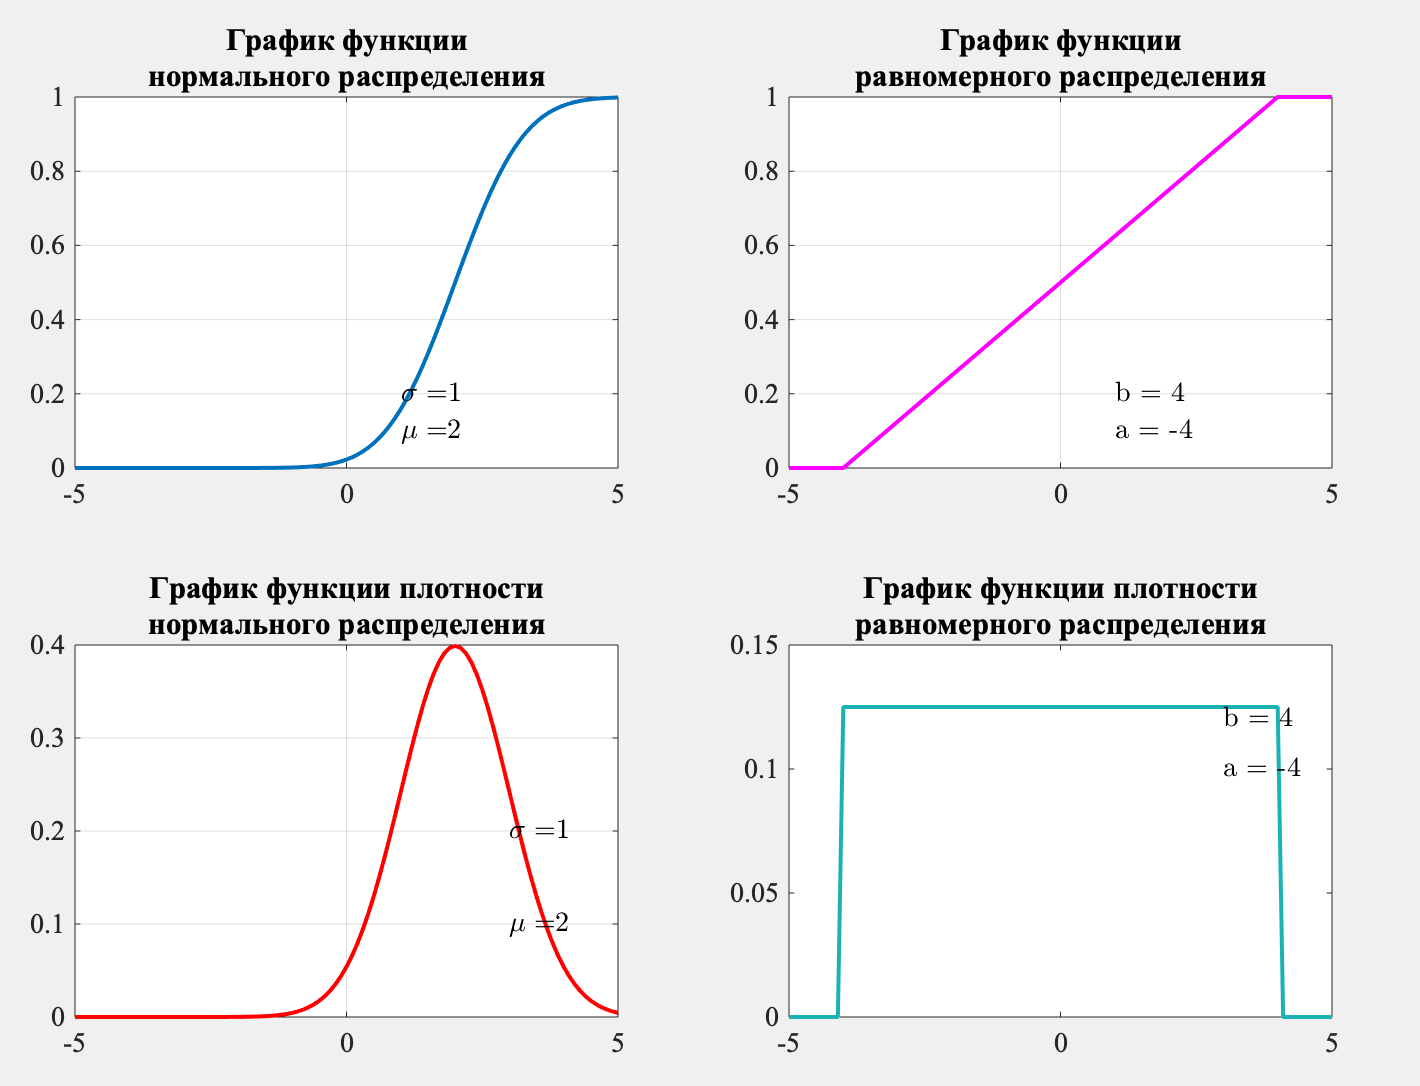
\includegraphics[scale=0.6]{1}
\end{figure}

\begin{figure}[H]
  \centering
  \caption{Пример 3. }
  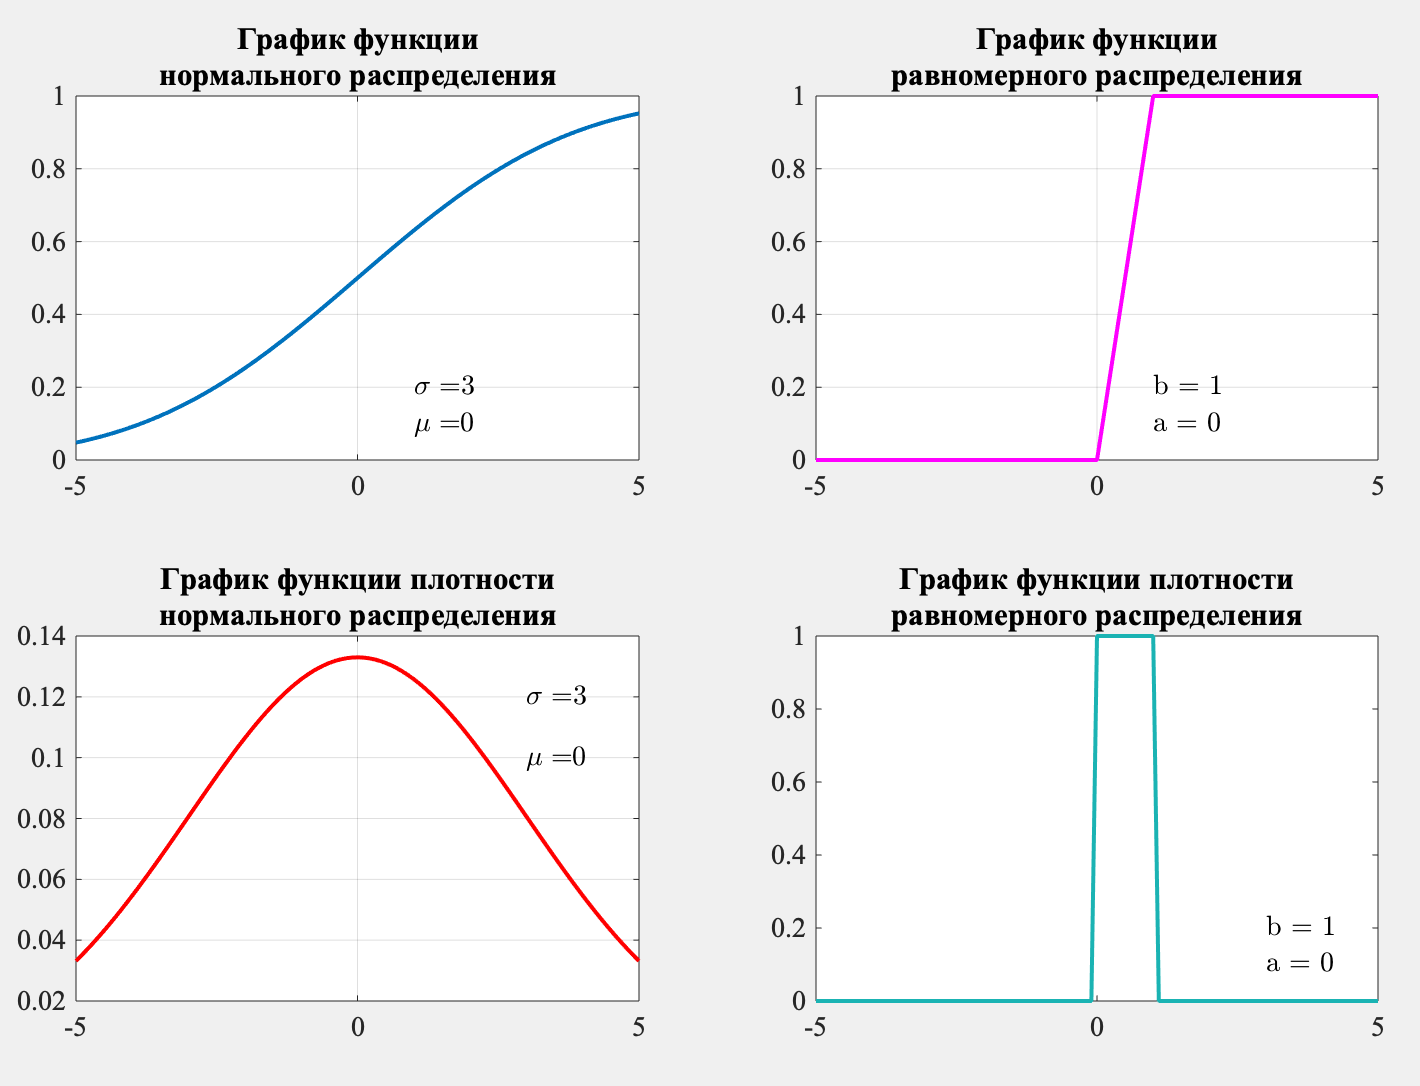
\includegraphics[scale=0.6]{3}
\end{figure}

\item \textbf{Вывод. }

Была написана программа для построения графиков функции и плотности распределения. Были построены графики при разных значениях параметров $\mu, \sigma$ для нормального распределения и $a, b$ для равномерного. 

\end{enumerate}
\end{document}